\documentclass[12pt]{article}
\usepackage{amssymb}
\usepackage{amsfonts}
\usepackage{amsthm}
\usepackage{amsmath}
\usepackage{setspace}
\usepackage{pstricks}
\usepackage{multirow}
\usepackage{geometry}
\usepackage{graphics}
\usepackage{booktabs, threeparttable, stackengine}
\usepackage{array}
\setstackgap{L}{12pt}
%\geometry{
%, left=1.25 in
%, right=1.25 in
%, top=1.4375 in
%, bottom=1.5 in}
\usepackage[pdftex]{graphicx}
\setcounter{MaxMatrixCols}{10}
\setlength{\textwidth}{6.5 in}
\setlength{\oddsidemargin}{0 in}
\setlength{\textheight}{8.5 in}
\setlength{\topmargin}{-0.1in}
\renewcommand\baselinestretch{1.5}
\makeatletter 
\def\@biblabel#1{\hspace*{-\labelsep}}
\makeatother 
\usepackage{hyperref}
\hypersetup{
	colorlinks=true,
	linkcolor=blue,
	filecolor=magenta,
	urlcolor=cyan,
}
\usepackage{stackengine}
\usepackage{graphicx}
\usepackage[scientific-notation=true]{siunitx}
\usepackage[numbers]{natbib}
\RequirePackage{filecontents}
\usepackage{float}
\begin{filecontents}{brexit.bib}
@article{begg:2016,
  title={The economic impact of brexit: jobs, growth and the public finances},
  author={Begg, Iain and Mush{\"o}vel, Fabian},
  year={2016},
  journal={The London School of Economics and Political Science, European Institute},

}
@article{corsmuel:2016,
  title="The pound and the macroeconomic effects of Brexit",
  author="Corsetti, Giancarlo and M{\"u}eller, Gernot",
  journal="VOX",
  year="2016"
}
@article{dhinetal:2016,
  title={The consequences of Brexit for UK trade and living standards},
  author={Dhingra, Swati and Ottaviano, Gianmarco IP and Sampson, Thomas and Reenen, John Van},
  year={2016},
  journal={London School of Economics and Political Science, CEP},
}
@article{heriponc:2015,
  title={Exchange rate volatility, financial constraints, and trade: empirical evidence from Chinese firms},
  author={H{\'e}ricourt, J{\'e}r{\^o}me and Poncet, Sandra},
  journal={The World Bank Economic Review},
  volume={29},
  number={3},
  pages={550--578},
  year={2015},
  publisher={World Bank}
}
@article{krugman:2014,
author="Krugman, Paul",
title="Currency Regimes, Capital Flows, and Crises",
journal="IMF Economic Review",
year="2014",
volume="62",
number="4",
pages="470--493",
}
@article{loretan:2005,
  title={Indexes of the foriegn exchange value of the dollar},
  author={Loretan, Mico},
  journal={Fed. Res. Bull.},
  volume={91},
  pages={1},
  year={2005},
  publisher={HeinOnline}
}
@article{olivwill:2016,
  title={Special relationships in flux: Brexit and the future of the US--EU and US--UK relationships},
  author={Oliver, Tim and Williams, Michael John},
  journal={International Affairs},
  volume={92},
  number={3},
  pages={547--567},
  year={2016},
  publisher={Wiley Online Library}
}
\end{filecontents}
\bibliographystyle{plainnat}
\begin{document}

\title{The Macroeconomic Impact of Brexit on the United States%
\thanks{%
I thank Dr. Uluc Aysun and Dr. Sami Alpanda for helpful comments on vector auto regression models and their guidance throughout the research process.}}
\date{First Version: August 20, 2016\\
This Version: December 13, 2016}
\author{Joshua Eubanks\thanks{%
Undergraduate Student, Department of Economics, University of Central Florida. 4336 Scorpius St.,
Orlando, FL 32816. \href{mailto:joshua.eubanks@knights.ucf.edu}{joshua.eubanks@knights.ucf.edu}}}
\maketitle
\thispagestyle{empty}
\begin{abstract}

This paper applies macroeconomic principles and current research to predict how Britain's economy will be in the future and how their future standing in the world economy will impact the United States in terms of investment, exchange rates, growth, trade, and labor. Using summary statistics, there does not seem to be a significant connection between the US and the UK. Additionally, there do not seem to be any indicators that the market perceives a recession, nor is there any significance in US GDP when exchange rates change. If the UK were to go into a fairly significant recession, there would be a negative impact to the US in later time periods.\\ 

\noindent \textit{Keywords}: Brexit, trade, vector auto regression, GDP growth, yield, exchange rates 

\setcounter{page}{0}\thispagestyle{empty}
\end{abstract}
\newpage
\section{Introduction}
There has been a lot of uncertainty post-Brexit, and investors are concerned with the United States' connection with the United Kingdom. This paper highlights the key indicators of their relationship:  exchange rates, growth rates, trade, labor, investment, and foreign-held assets. Correlation and variance are calculated for GDP growth, yield curve slopes, and exchange rates. Using the trade and foreign-held assets information, the extreme cases in terms of trade and foreign-held assets are presented. Lastly, a vector auto regressive model is built and shocks are implemented to UK growth rates and US/UK exchange rates to observe how the US's growth, inflation, and interest rates are affected.\\

There has been little published research about the implications Brexit will have upon the US. A paper by \citet{olivwill:2016} acknowledges the US-UK relationship and how that relationship impacts the US-EU relationship. In the ``bad'' scenario of the paper\footnote{In the conclusion there are three outcomes: the good, the bad, and the ugly.} it states that post-Brexit, the UK and the EU would become more difficult to negotiate with since the UK is a sort of ``transatlantic bridge'' in terms of relationships between the US and EU. In this paper, it is shown that even if all exports stopped with the EU and the UK, it would only impact the US GDP by less than 1$\%$. In the ``ugly'' section the authors propose that after post-Brexit, other countries may be inclined to leave the EU as well, thereby causing an unraveling of the EU. This is not considered in this paper as it would seem rather unlikely for this to occur.\\

More research has been into the effects on the UK post-Brexit. \citet{dhinetal:2016} state that under the dynamic case Brexit will cause a decline in household income by 6.3$\%$ in the optimistic case and 9.5$\%$ in the pessimistic case in the long run. The paper also shows that there would not be a decrease in living standards for the US. \citet{begg:2016} state that similar predictions such as the one by \citet{dhinetal:2016} do not account for the growth rate of the UK, which is projected to be 30$\%$ larger by 2030 based on the current trend rate. This paper also finds that there will be no significant impact of Brexit on the US.     

\section{UK's Economic Status}
As the level of uncertainty increases, the pound depreciates. There is a consensus that as the pound depreciates, exports will rise. Alternatively, there does not seem to be a clear answer about whether or not domestic output would rise. \citet{krugman:2014} suggests that domestic output would rise because the export boom will outweigh the reduction in internal demand. \citet{corsmuel:2016} refute this claim by stating that in order for this to work, the UK would need effective monetary policy. Ideally, the central bank would want to increase the monetary supply thus reducing interest and exchange rates to increase net exports and domestic financing; however, Britain cannot do this because they're already at the zero lower bound (liquidity trap).\\ 

Two basic tools are implemented in this paper to observe how the market perceives future growth: the yields on UK government bonds and the price-to-earning ratio. Data was collected from Bloomberg on the UK and US government bonds for 1, 5, 10, 15, and 30 year generic bid yield. Data was also collected on the yearly reported price-to-earnings ratios of the top 4 British companies in terms of market cap in 2008: Shell, BP, HSBC, and GlaxoSmithKline from the Bloomberg database.  
\subsection{Yield}
The yield curves for UK government bonds have not been ``flattening'' over the past year, indicating that Britain may not face a recession. If investors believed that the UK was headed towards a recession, the yield on a 1-year bond would increase by a greater amount than the long term bond yields. In Figure \ref{yield}, it is shown that the yield curves in the past 4 quarters have remained relatively stable.\\

Another tool that is used is the approximate slope of the yield curve ($\dfrac{i_{30}-i_{1}}{30}$). Using data from 11/17/2015 - 11/17/2016, the slope was calculated for each market day. As Figure \ref{slope} shows, there was a slight decrease around the time of Brexit; however, the slope has been increasing afterwards. Additionally, the slope is plotted for the US generic bid yield to illustrate the movement between both slopes.


\subsection{P/E Ratio}
Another measure of the economy is the price-to-earning ratio for British corporations. Shell and BP are petrol, oil, extraction companies, HSBC is a banking institution, and GlaxoSmithKline is a pharmaceutical company. As it is shown in Figure \ref{pe} below, there has not been a significant drop in the P/E ratio, and it is not projected to fall by a significant amount by 2020\footnote{The last reported yearly P/E ratio is 2015, projections provided by Bloomberg start at 2016. HSBC reports yearly P/E ratio around the beginning of March. All others report around the beginning of February.}. A drop in the P/E ratio would signal that the market expects to have less earnings on those investments. 

%\section{The pound and the macroeconomic effects of Brexit}
%The authors make the argument that if Britain decides to leave the EU, the pound would become relatively weaker and will be more volatile for a long period of time because of how interconnected they are with the EU. They refute the claim that is made by Krugman that the export boom (due to the depreciation in exchange rates) will outweigh the uncertainty thereby not causing a reduction in domestic output. They refute this claim by showing that in order for this to work, they need effective monetary policy. Ideally, the central bank would want to increase the monetary supply thus reducing interest and exchange rates to increase net exports and domestic financing, however, Britain cannot do this because they're already at the zero lower bound (liquidity trap). The authors also create a model to illustrate their point. In the model, they implement a shock to the market (increase in risk premium) and show the changes in six variables. They show the changes to these six variables and observe the differences in each when there is a monetary policy, and one when they do not implement any monetary measures. It shows that it is true that domestic output would slightly increase with monetary policy action, however, it will decrease without any monetary policy. Since the most effective monetary policy cannot be used in the case of Britain, the authors argue that the second scenario is more likely to occur.

\section{Impact on US economy}
This section investigates the link between the US and the UK. If the UK were to go into a recession, how would that impact the US now that the UK is not part of the EU? To analyze this question, the data collected from the FRED database was split into two time periods: before Britain joined the EMU (1980-1999) denoted with a subscript $i$, and after (1999-2015) denoted as a subscript $c$. A ``control'' factor is implemented in both models and the ratio is taken within both time periods to account for globalization. Trade, foreign-held assets, and migration are observed and then the two extreme sides of the spectrum in terms of trade are observed to consider the possible impact on US GDP.  

\subsection{Variability in Exchange Rates}\label{variance}
\citet{heriponc:2015} find that firms export less to countries that have higher exchange rate volatility. Looking at the variance of the US-UK exchange rate will allow us to make statements about future trade patterns. Additionally, an increase in exchange rate variance may cause a decline in investment between the the two countries since the return on an investment is not as certain.\\

To account for the reduction in variance due to globalization, the trade weighted U.S. dollar index denoted as $\omega_j$ where $j = i,c$ is used as the  ``control'' factor. $\omega$ will account for globalization because the trade weighted index aligns close with US trade patterns. Variance for the trade weighted USD index will decrease due to globalization, thereby offsetting some of the reduction in the exchange rate due to globalization. The reduction in the variance is due to the fact that five of the ten currencies in the index before the EMU were replaced by the Euro (\citet{loretan:2005}).\\

Since $\mathbb{X}_{j} = \mathbb{V}\left(\dfrac{\$_{j}}{\pounds_{j}}\right)$ where $j = i,c$ then as $\mathbb{V}\left(\dfrac{\$_{i}}{\pounds_{i}}\right) = \num{0.05967598}$, $\mathbb{V}\left(\dfrac{\$_{c}}{\pounds_{c}}\right) = \num{0.02832951}$ and $\mathbb{V}(\omega_i) = \num{222.135}, \mathbb{V}(\omega_i) = \num{147.4268}$, $\mathbb{X}_{i} = \num{0.0002686474}$ and $\mathbb{X}_{c} = \num{0.0001921598}$ therefore, $\mathbb{X}_{i} > \mathbb{X}_{c}$. This states that the variance of the $\dfrac{\$}{\pounds}$ rate is higher before Britain joined the EMU. This is logical because Britain had to tie their exchange rates closely to the EU thus reducing the pound's variance. Now that Britain has left the EMU, they will no longer have to tie their exchanges rates closely to the Euro. Since Britain is leaving the EMU, it is possible to expect the rates to fluctuate more after Brexit therefore we may expect to see a decline in trade and investment between the US and the UK. 
%\begin{align*}
%\dfrac{\mathbb{V}\left(\dfrac{\$_{i}}{\pounds_{i}}\right)}{\mathbb{V}(\omega_i)} &> \dfrac{\mathbb{V}\left(\dfrac{\$_{c}}{\pounds_{c}}\right)}{\mathbb{V}%%(\omega_c)}\\[5pt]
%\dfrac{\num{0.05967598}}{\num{222.135}}&>\dfrac{\num{0.02832951}}{\num{147.4268}}\\
%\mathbb{X}_{i} &> \mathbb{X}_{c}
%\end{align*}
%Implementing R for the calculations, the value for $\mathbb{X}_{i} = \num{0.0002686474}$ and $\mathbb{X}_{c} = \num{0.0001921598}$.\\

\subsection{Correlation of Growth Rates}
After the UK joined the EMU, the correlation between the US growth rates ($y^{us}_c$) and the growth rates of the UK ($y^{uk}_c$) was stronger than before the UK joined the EMU. The control factor is the correlation between the US growth rates and the G7 GDP growth rate ($y^{g7}_{n}$ $where$ $n=i,c$).\\

Since $\mathbb{G}_{j} = \dfrac{cor(y^{us}_j,y^{uk}_j)}{cor(y^{us}_j,y^{g7}_j)}$ where $j = i,c$ then as $cor(y^{us}_i,y^{uk}_i) = 0.3302727$,\\ $cor(y^{us}_c,y^{uk}_c) = 0.6180597$ and $cor(y^{us}_i,y^{g7}_i) = \num{222.135}, cor(y^{us}_c,y^{g7}_c) = 0.879261$,\\ $\mathbb{G}_{i} = 0.3876888$ and $\mathbb{G}_{c} = 0.702931$ therefore, $\mathbb{G}_{i} < \mathbb{G}_{c}$.
%\begin{align*}
%\dfrac{cor(y^{us}_i,y^{uk}_i)}{cor(y^{us}_i,y^{g7}_i)} &< \dfrac{cor(y^{us}_c,y^{uk}_c)}{cor(y^{us}_c,y^{g7}_c)}\\[5pt]
%\dfrac{0.3302727}{0.8519016}&< \dfrac{0.6180597}{0.879261}\\
%\mathbb{G}_{i} &< \mathbb{G}_{c}
%\end{align*}

%Implementing R, the value for $\mathbb{G}_{i} = 0.3876888$ and $\mathbb{G}_{c} = 0.702931$.\\

\subsection{Correlation of Yield Curve Slopes}
Using the data from Figure \ref{slope}, a correlation test was run between the percent change in the slope from the previous day for the US and the UK for the year\footnote{Stated more formally, $cor\left( \dfrac{s^{us}_t-s^{us}_{t-1}}{s^{us}_{t-1}},\dfrac{s^{uk}_t-s^{uk}_{t-1}}{s^{uk}_{t-1}}\right)$ where $s$ denotes the slope.} A relation of 0.4632338 was found, which indicates a significant relationship between them. Additionally, a lag correlation was implemented to determine if one slope may be strongly correlated with another in different time periods, but as Figure \ref{lagyield} shows, it appears that the strongest correlation is in the same time period.


\subsection{Trade}
Data was collected on exports and imports for both UK and the US from the MIT's observatory of economy complexity in the year 2014. Two extremes cases are presented. The first was what if, post-Brexit, it has become more expensive for the UK to import from members in the EU due to trade restrictions, thereby making it cheaper to import from the US, so much cheaper that it diverts all imports from the EU and only imports from the US. As Table \ref{trade} shows, 56$\%$ of the UK's imports are from the EU. This would increase the US GDP by approximately 373 billion dollars or 25.7$\%$ of total exports or 2.15$\%$ of total US GDP.\\

Another extreme case would be one in which the purchasing power of the pound has decreased such a significant amount that now all of the members of the EU decide to import exclusively from the UK. This would cause a decline in exports for the US by 239 billion dollars or 16.5$\%$ of total net exports. If UK also finds it less costly to import from the EU exclusively, exports for the US would fall by an additional 3$\%$. This would reduce US GDP by .1635$\%$.

\subsection{Labor Mobility and Foreign-held Securities}
If the pound becomes less valuable, it may become less expensive for  US citizens to migrate to the UK and it may become more expensive for UK citizens to migrate to the US.
In 2015 714,999 (1.1$\%$ of the UK population) individuals whose origin was in the UK now live in the US, and 212,150 (.066$\%$ of the US population)\footnote{Population estimates for the UK and US were provided by the Office for National Statistics and the US Census Bureau respectively.} of US native individuals migrated to the UK. This does not indicate a significant amount of connection in terms of migration for the US because migration to the UK only accounts for 7$\%$ of all outward migration from the US, but migration from the UK to the US accounts for 15.6$\%$ of all migration from the UK\footnote{Source: United Nations database, POP/DB/MIG/Stock/Rev.2015}. \\

In the case of a depreciation of the pound, the US would not make as much of a return on their investments in the UK. Similar to a increase in inflation in a domestic investment, the lender (in this case, the US) would have less return because the real value of the debt will be less. Additionally, UK investment into the US would increase because the real rate of return increases when the investor's currency depreciates.
Figure \ref{foreign} shows the 2015 market value of U.S. portfolio holdings of foreign securities. As it is shown, only 13$\%$ of the US's portfolio is in London. Furthermore, approximately 27.7$\%$ of the UK securities are in long-term and short-term debt. Even if the UK defaulted on all of its debt, it would only impact the US's portfolio by 3.6 $\%$. Figure \ref{investment} shows the net foreign purchases of US securities from the UK. One thing in particular that stands out is the increase in the foreign bonds category. This may be due to an increase in investment from the UK or a decrease in investment from the US. If it is a decrease in investment from the US, it could be the case that the impact would be smaller if the UK defaulted on its debt. 

\section{VAR Model}
Quarterly data was collected from the Bloomberg database spanning from Q2 1989 - Q2 2016. The characteristics of the data are as follows: For US inflation US CPI Urban Consumers YoY NSA (CPI YOY:IND); the UK inflation the UK CPI EU Harmonized YoY NSA (UKRPCJYR:IND); for growth rates for both countries, the FRED database was used; for interest rates for the US ICAP US Federal Funds Rate (FDFD:IND); for UK interest rates the immediate rates less than 24 hours (IRSTCI0IGBQ156N); exchange rate data was the same data from section 3.1 and the quarterly average was calculated\footnote{In the FRED database, quarterly data was reported at the first of the month, whereas in the Bloomberg database, quarters were reported on the last day of the month. Ex: Q3 2016 from the Bloomberg database was reported as 9/30/2016 and it was reported as 10/1/2016 in the FRED database.}. The purpose of the VAR is to explain how sensitive the US macro variables are to shocks in changes in UK variables. 
\subsection{Structure}
Using Cholesky ordering, the structure of the model is as follows:
\begin{align*}
\begin{bmatrix}
\Pi^{us}\\
\Pi^{uk}\\
y^{us}\\
y^{uk}\\
i^{us}\\
i^{uk}\\
e
\end{bmatrix}
\end{align*}
The model is set in this manner because the assumption is that the US has a stronger impact on the UK economy than the UK has on the US, so setting $\Pi^{us}$ before $\Pi^{uk}$ implies that a change in US inflation would directly impact UK inflation in the same period, but a change in UK inflation would only have an impact in future time periods. Additionally, setting inflation first assumes that growth rates do not directly impact inflation, but rather impact inflation in future periods, but inflation directly impacts US growth. This continues for all other variables in the model.
\subsection{FEVD}
Table \ref{fevd} shows the variance decomposition of the variables within the model for time periods one quarter in advance to 2 years in advance. In $t+1$, it shows that when a using an ordered VAR, the model doesn't explain how much of the forecasting error is explained by exogenous shocks to variables that are after the variable we are trying to forecast. This is a limitation to this sort of structure. 
Two years ahead, we can tell that 10\% of the forecasting error in US GDP growth rates can be explained by an exogenous shock to UK GDP growth rates. Additionally, only .4\% of the variance in the forecast error can be explained by a shock to the exchange rates. This shows that US-UK exchange rates do not have a significant impact on explaining any changes in US growth rates. 
\subsection{Identifying Shocks}
One test that was implemented to check the validity of the shocks were simplified models, one as $\Pi^{us}$, $y^{us}$, and $i^{us}$ and the other model the same, but the UK variables were used in the second model. The purpose behind this was to ensure that responses of these shocks follow economic principles (e.g. an increase in GDP growth will increase interest rates and inflation). As Figures \ref{yus} and \ref{yuk} show, these shocks do follow the basic structure.
\subsection{Full Models}
Now that the responses are validated, models are built to show the how the decrease in output growth for the UK and a separate model that shows a shock to exchanges rates to observe how the variables above react to these shocks. As Figure \ref{irfex} shows, an increase in the exchange rates has no significant impact on US GDP growth rates; it will slightly decrease US inflation but increases UK inflation. In Figure \ref{irfuk}, an increase to UK GDP growth have a significant impact to US GDP growth rates and inflation in the same direction\footnote{The question posed in this paper is the impact of a negative shock to $y^{uk}$. I was unable to model that in R; however, the effects would be mirrored if it were a negative shock and the upper CI would be the lower and vice versa.}.\\

\section{Conclusion}
There does not seem to be any evidence that suggests that Brexit will have a significant impact on the US at this time. In \citet{corsmuel:2016}, one of the main concerns post-Brexit is a currency collapse. In the VAR, the $\dfrac{\$}{\pounds}$ exchange rate did not have a significant impact on US GDP. Additionally, although the VAR does show that a negative output gap could impact the US in future time periods, the market does not expect a reduction in UK GDP growth.\\

In this paper, the EU is not considered as some underlying factor that may be adding an effect to growth rates. It could be the case, that if the UK goes into a recession, it may affect the EU negatively as well, thereby impacting the US GDP growth. This will be addressed in future revisions.
\newpage
\section*{Tables and Figures}

\begin{table}[!htbp] \centering 
  \caption{Exports and Imports for the US and the UK} 
\scalebox{.75}{
\makebox[\linewidth]{ 
  \label{trade} 
\begin{tabular}{@{\extracolsep{5pt}} ccccccccc} 
\\[-1.8ex]\hline 
\hline \\[-1.8ex] 
Country & US Exports &  & US Imports &  & UK Exports &  & UK Imports &  \\\hline \\[-1.8ex]
 & \$ (in trillions) & \% & \$ (in trillions) & \% & \$ (in billions) & \% & \$ (in billions) & \% \\ 
Austria & 0.00549 & 0.379\% & 0.0104 & 0.475\% & 2.77 & 0.586\% & 5.24 & 0.789\% \\ 
Belgium-Luxembourg & 0.03400 & 2.345\% & 0.0165 & 0.753\% & 22.1 & 4.672\% & 35.3 & 5.316\% \\ 
Bulgaria & 0.00038 & 0.026\% & 0.000544 & 0.025\% & 0.578 & 0.122\% & 6.48 & 0.976\% \\ 
Croatia & 0.00039 & 0.027\% & 0.000385 & 0.018\% & 0.295 & 0.062\% & 0.179 & 0.027\% \\ 
Republic of Cyprus & 0.00010 & 0.007\% & 0.00007 & 0.003\% & 0.514 & 0.109\% & 0.282 & 0.042\% \\ 
Czech Republic & 0.00358 & 0.247\% & 0.00418 & 0.191\% & 3.29 & 0.696\% & 8.1 & 1.220\% \\ 
Denmark & 0.00246 & 0.170\% & 0.00762 & 0.348\% & 4.68 & 0.989\% & 7.78 & 1.172\% \\ 
Estonia & 0.00039 & 0.027\% & 0.000636 & 0.029\% & 0.619 & 0.131\% & 0.377 & 0.057\% \\ 
Finland & 0.00286 & 0.197\% & 0.0052 & 0.237\% & 2.32 & 0.490\% & 3.91 & 0.589\% \\ 
France & 0.03930 & 2.710\% & 0.0403 & 1.840\% & 27 & 5.708\% & 41.5 & 6.250\% \\ 
Germany & 0.06160 & 4.248\% & 0.121 & 5.525\% & 46.5 & 9.831\% & 100 & 15.060\% \\ 
Greece & 0.00067 & 0.046\% & 0.00104 & 0.047\% & 1.61 & 0.340\% & 1.28 & 0.193\% \\ 
Hungary & 0.00200 & 0.138\% & 0.00488 & 0.223\% & 1.67 & 0.353\% & 4.12 & 0.620\% \\ 
Ireland & 0.00745 & 0.514\% & 0.0285 & 1.301\% & 24.3 & 5.137\% & 19.2 & 2.892\% \\ 
Italy & 0.01640 & 1.131\% & 0.0408 & 1.863\% & 13.4 & 2.833\% & 28.1 & 4.232\% \\ 
Latvia & 0.00018 & 0.012\% & 0.000248 & 0.011\% & 0.306 & 0.065\% & 0.704 & 0.106\% \\ 
Lithuania & 0.00062 & 0.043\% & 0.0011 & 0.050\% & 1.39 & 0.294\% & 1.6 & 0.241\% \\ 
Malta & 0.00081 & 0.056\% & 0.000175 & 0.008\% & 0.536 & 0.113\% & 0.221 & 0.033\% \\ 
Netherlands & 0.03460 & 2.386\% & 0.0198 & 0.904\% & 34.2 & 7.230\% & 50.7 & 7.636\% \\ 
Poland & 0.00517 & 0.357\% & 0.00522 & 0.238\% & 5.63 & 1.190\% & 13 & 1.958\% \\ 
Portugal & 0.00122 & 0.084\% & 0.00307 & 0.140\% & 2.41 & 0.510\% & 3.83 & 0.577\% \\ 
Romania & 0.00095 & 0.065\% & 0.00196 & 0.089\% & 1.69 & 0.357\% & 2.57 & 0.387\% \\ 
Slovakia & 0.00086 & 0.059\% & 0.00199 & 0.091\% & 1.02 & 0.216\% & 3.87 & 0.583\% \\ 
Slovenia & 0.00062 & 0.043\% & 0.000641 & 0.029\% & 0.456 & 0.096\% & 0.585 & 0.088\% \\ 
Spain & 0.01320 & 0.910\% & 0.014 & 0.639\% & 14.5 & 3.066\% & 22 & 3.313\% \\ 
Sweden & 0.00399 & 0.275\% & 0.0102 & 0.466\% & 9.27 & 1.960\% & 12.3 & 1.852\% \\ 
United Kingdom & 0.04440 & 3.062\% & 0.051 & 2.329\% &  -    &  -    &  -    &  -    \\ 
United States &  -    &  -    &  -    &  -    & 51 & 10.782\% & 44.4 & 6.687\% \\ 
EU (without UK) & 0.23927 & 16.502\% &  0.34  & 15.543\% &  223.05  & 47.2\% & 373.22800 & 56.209\% \\ 
\hline \\[-1.8ex] 
\end{tabular} 
}}
\end{table}
\begin{table}[!htbp] \centering 
  \caption{Forecast Error Variance Decomposition for $t+1$ and $t+8$} 
  \label{fevd}
\begin{tabular}{@{\extracolsep{5pt}} cccccccc} 
\\[-1.8ex]\hline 
\hline \\[-1.8ex] 
          &$\Pi^{us}$& $\Pi^{uk}$&$y^{us}$&$y^{uk}$&$i^{us}$&$i^{uk}$& $e$\\ 
$\Pi^{us}_{t+1}$&    $1$   & $0$       & $0$     & $0$     & $0$    & $0$    & $0$ \\ 
$\Pi^{uk}_{t+1}$&$0.150$ & $0.850$ & $0$ & $0$ & $0$ & $0$ & $0$ \\ 
$y^{us}_{t+1}$ &$0.042$ & $0.0004$& $0.958$ & $0$ & $0$ & $0$ & $0$ \\ 
$y^{uk}_{t+1}$ &$0.037$ & $0.010$ & $0.096$ & $0.857$ & $0$ & $0$ & $0$ \\ 
$i^{us}_{t+1}$          &$0.041$ & $0.017$ & $0.044$ & $0.002$ & $0.896$ & $0$ & $0$ \\ 
$i^{uk}_{t+1}$          &$0.034$ & $0.036$ & $0.003$ & $0.001$ & $0.090$ & $0.836$ & $0$ \\ 
$e_{t+1}$          &$0.009$ & $0.008$ & $0.001$ & $0.017$ & $0.017$ & $0.004$ & $0.944$ \\\hline \hline \\[-1.8ex]
$\Pi^{us}_{t+8}$&$0.789$ & $0.105$ & $0.009$ & $0.040$ & $0.001$ & $0.017$ & $0.039$ \\ 
$\Pi^{uk}_{t+8}$&$0.146$ & $0.752$ & $0.036$ & $0.025$ & $0.005$ & $0.008$ & $0.029$ \\ 
$y^{us}_{t+8}$ &$0.035$ & $0.017$ & $0.804$ & $0.102$ & $0.020$ & $0.018$ & $0.004$ \\ 
$y^{uk}_{t+8}$ &$0.047$ & $0.071$ & $0.313$ & $0.533$ & $0.0004$ & $0.036$ & $0.0002$ \\ 
$i^{us}_{t+8}$          &$0.026$ & $0.022$ & $0.081$ & $0.070$ & $0.741$ & $0.047$ & $0.013$ \\ 
$i^{uk}_{t+8}$          &$0.027$ & $0.109$ & $0.077$ & $0.013$ & $0.070$ & $0.684$ & $0.020$ \\ 
$e_{t+8}$          &$0.055$ & $0.045$ & $0.045$ & $0.019$ & $0.025$ & $0.281$ & $0.530$ \\ 
\hline \\[-1.8ex] 
\end{tabular} 
\end{table} 
\begin{figure}[H]
\centering
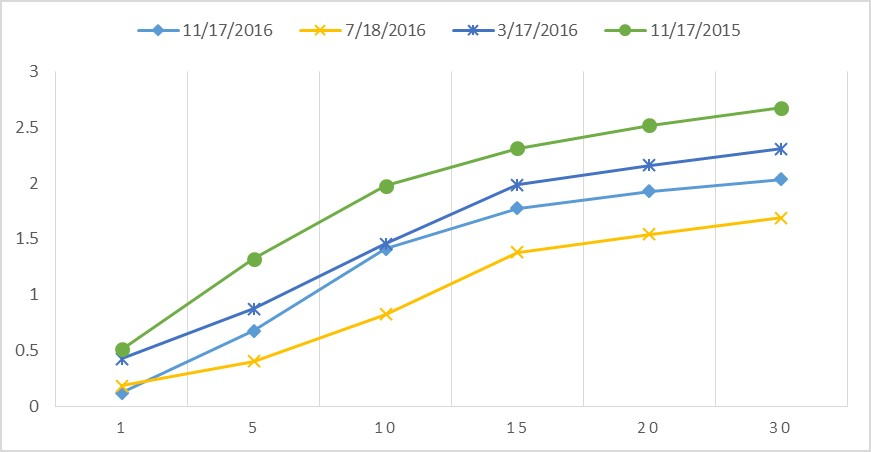
\includegraphics[scale=]{yield.jpg}
\caption{Yield Curves}\label{yield}
\end{figure}
\begin{figure}[H]
\centering
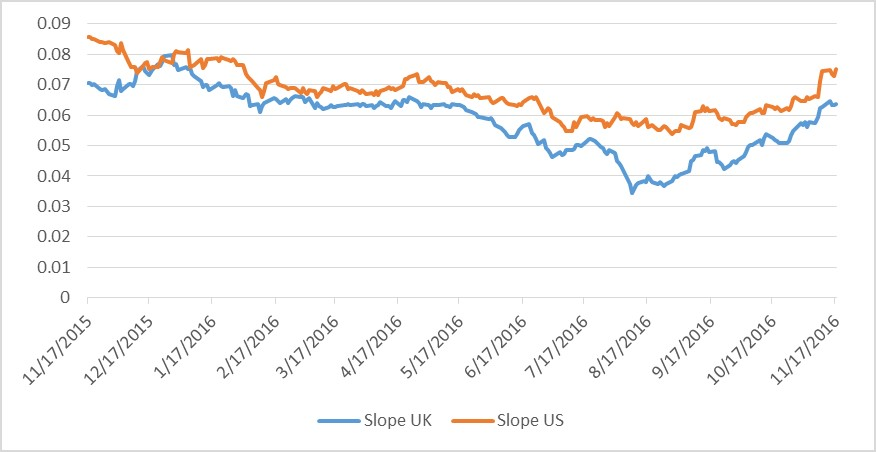
\includegraphics[scale=]{slope.jpg}
\caption{Slope of Yield Curves} \label{slope}
\end{figure}
\begin{figure}[H]
\centering
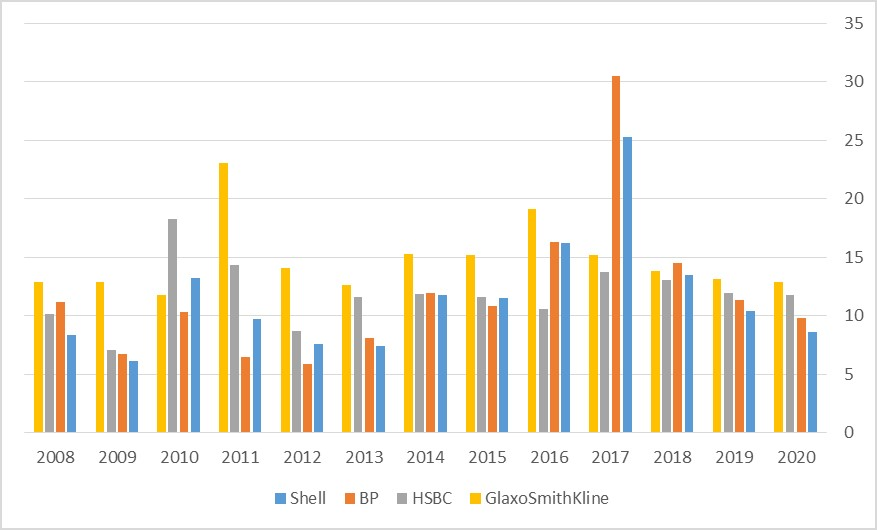
\includegraphics[scale=]{pe.jpg} 
\caption{P/E Ratios}\label{pe}
\end{figure}
\begin{figure}[H]
\centering
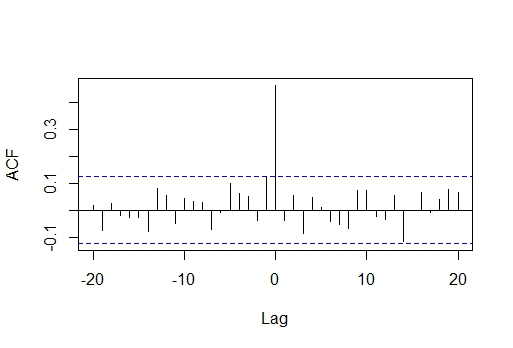
\includegraphics[scale=.65]{lagyield.jpeg}
\caption{Lag correlations between US and UK yield slopes.} \label{lagyield}
\end{figure}
\begin{figure}[H]
\centering
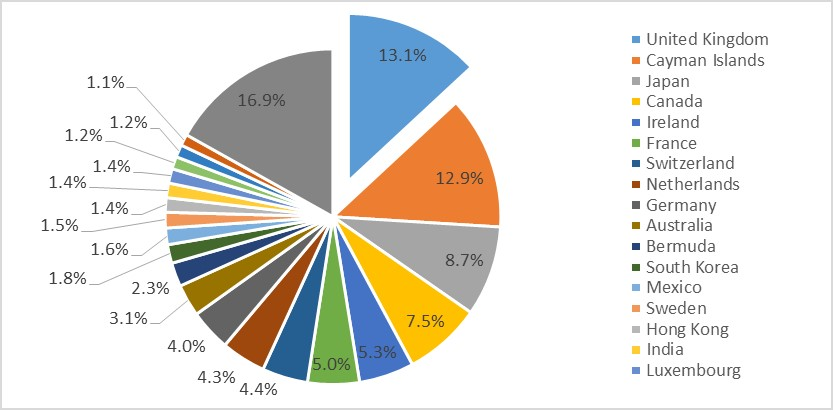
\includegraphics[scale=]{foreign.jpg}
\caption{2015 market value of U.S. portfolio holdings of foreign securities by country as reported by the Treasury.}\label{foreign}
\end{figure}
\begin{figure}[H]
\centering
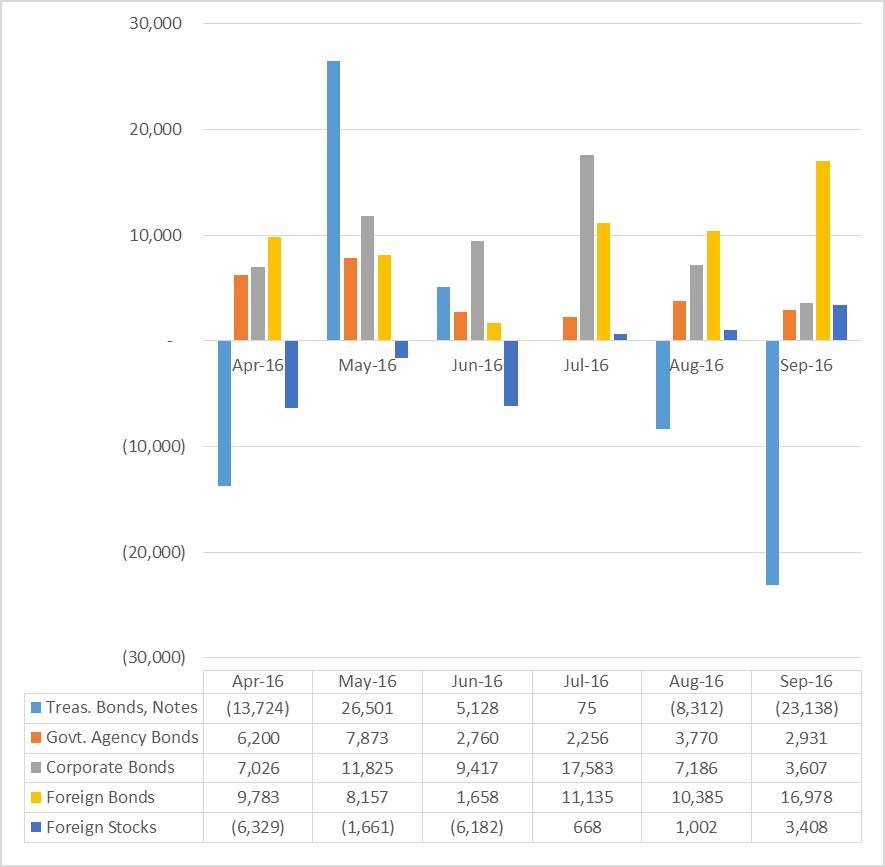
\includegraphics[scale=]{investment.jpg} 
\caption{Net Foreign Purchases of US Securities by the United Kingdom (in millions)}\label{investment}
\end{figure}
\begin{figure}[H]
\centering
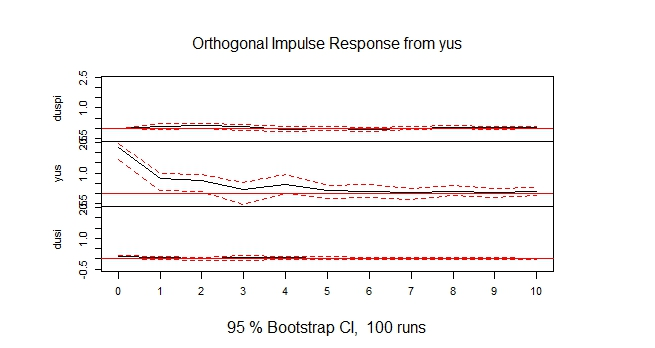
\includegraphics[scale=.8]{yus.jpeg} 
\caption{Impulse response functions when a shock is applied to US growth rates in the simplified model}\label{yus}
\end{figure}
\begin{figure}[H]
\centering
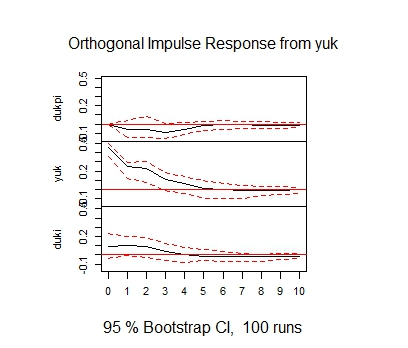
\includegraphics[scale=.8]{yuk.jpeg} 
\caption{Impulse response functions when a shock is applied to UK growth rates in the simplified model}\label{yuk}
\end{figure}
\begin{figure}[H]
\centering
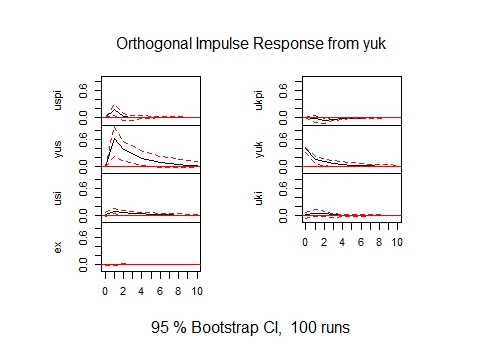
\includegraphics[scale=.8]{irfuk.jpeg} 
\caption{Impulse response functions when a shock is applied to UK growth rates}\label{irfuk}
\end{figure}
\begin{figure}[H]
\centering
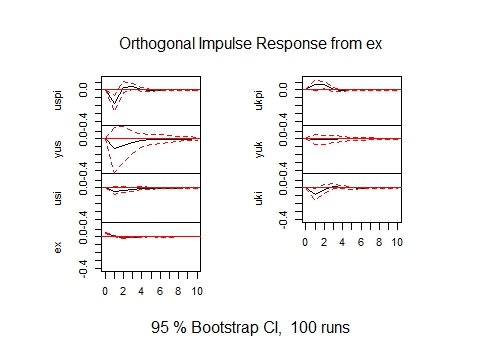
\includegraphics[scale=.85]{irfex.jpeg}  
\caption{Impulse response functions when a shock is applied to US/UK exchange rates}\label{irfex}
\end{figure}

\bibliography{brexit}
\end{document}